\chapter{نظریه بازی‌ها}

در این فصل، روی بازی‌های دو نفره بدون عامل شانس تمرکز می‌کنیم.
هدف یافتن راهبردی است که در صورت وجود،
پیروزی ما را مستقل از حرکت‌های حریف
تضمین کند.

یک راهبرد کلی برای چنین بازی‌هایی وجود دارد
و تحلیل آن‌ها با استفاده از \key{نظریه نیم} (nim theory) امکان‌پذیر است.
ابتدا بازی‌های ساده‌ای بررسی می‌شوند که در آن‌ها
بازیکنان چوب‌ها را از کپه‌ها برمی‌دارند؛
سپس این راهبرد به بازی‌های دیگر تعمیم داده می‌شود.

\section{وضعیت‌های بازی}

بازی با یک کپه شامل $n$ چوب را در نظر بگیرید.
بازیکنان $A$ و $B$ به نوبت بازی می‌کنند
و شروع با بازیکن $A$ است.
در هر نوبت، بازیکن باید
۱، ۲ یا ۳ چوب از کپه بردارد.
بازیکنی که آخرین چوب را بردارد برنده است.

به عنوان مثال، اگر $n=10$ باشد، روند بازی می‌تواند چنین باشد:
\begin{itemize}[noitemsep]
\item بازیکن $A$ تعداد ۲ چوب برمی‌دارد (۸ چوب باقی می‌ماند).
\item بازیکن $B$ تعداد ۳ چوب برمی‌دارد (۵ چوب باقی می‌ماند).
\item بازیکن $A$ تعداد ۱ چوب برمی‌دارد (۴ چوب باقی می‌ماند).
\item بازیکن $B$ تعداد ۲ چوب برمی‌دارد (۲ چوب باقی می‌ماند).
\item بازیکن $A$ تعداد ۲ چوب برمی‌دارد و برنده می‌شود.
\end{itemize}

این بازی از وضعیت‌های $0,1,2,\ldots,n$ تشکیل شده است،
که در آن شماره وضعیت نشان‌دهنده
تعداد چوب‌های باقی‌مانده است.

\subsubsection{وضعیت‌های برنده و بازنده}

\index{وضعیت برنده}
\index{وضعیت بازنده}

یک \key{وضعیت برنده} وضعیتی است که
اگر بازیکن بهینه بازی کند،
برنده خواهد شد.
یک \key{وضعیت بازنده} وضعیتی است
که در صورت بازی بهینه حریف،
بازیکن بازنده خواهد شد.
می‌توان تمام وضعیت‌های بازی را به‌گونه‌ای دسته‌بندی کرد
که هر وضعیت یا برنده باشد یا بازنده.

در بازی بالا، وضعیت ۰ مشخصاً یک
وضعیت بازنده است، چون بازیکن نمی‌تواند
حرکتی انجام دهد.
وضعیت‌های ۱، ۲ و ۳ وضعیت‌های برنده هستند،
زیرا می‌توان ۱، ۲ یا ۳ چوب برداشت
و بازی را برد.
وضعیت ۴ به نوبه خود یک وضعیت بازنده است،
زیرا هر حرکتی به وضعیتی منجر می‌شود که
برای حریف یک وضعیت برنده است.

به‌طور کلی، اگر حرکتی از وضعیت فعلی
به یک وضعیت بازنده وجود داشته باشد،
وضعیت فعلی برنده است؛
در غیر این صورت، وضعیت فعلی بازنده است.
با استفاده از این قاعده، می‌توان تمام وضعیت‌های یک بازی را
با شروع از وضعیت‌های بازنده‌ای که حرکتی در آن‌ها ممکن نیست دسته‌بندی کرد.

وضعیت‌های $0 \ldots 15$ بازی بالا
را می‌توان به شکل زیر دسته‌بندی کرد
($W$ نشان‌دهنده وضعیت برنده و $L$ نشان‌دهنده وضعیت بازنده است):
\begin{center}
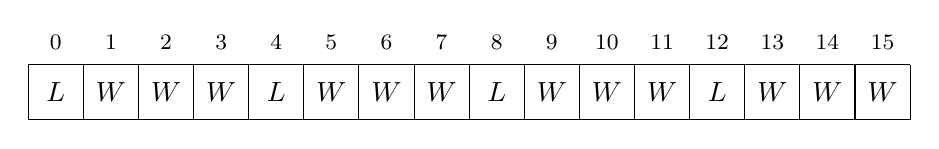
\begin{tikzpicture}[scale=0.7]
\draw (0,0) grid (16,1);

\node at (0.5,0.5) {$L$};
\node at (1.5,0.5) {$W$};
\node at (2.5,0.5) {$W$};
\node at (3.5,0.5) {$W$};
\node at (4.5,0.5) {$L$};
\node at (5.5,0.5) {$W$};
\node at (6.5,0.5) {$W$};
\node at (7.5,0.5) {$W$};
\node at (8.5,0.5) {$L$};
\node at (9.5,0.5) {$W$};
\node at (10.5,0.5) {$W$};
\node at (11.5,0.5) {$W$};
\node at (12.5,0.5) {$L$};
\node at (13.5,0.5) {$W$};
\node at (14.5,0.5) {$W$};
\node at (15.5,0.5) {$W$};

\footnotesize
\node at (0.5,1.4) {$0$};
\node at (1.5,1.4) {$1$};
\node at (2.5,1.4) {$2$};
\node at (3.5,1.4) {$3$};
\node at (4.5,1.4) {$4$};
\node at (5.5,1.4) {$5$};
\node at (6.5,1.4) {$6$};
\node at (7.5,1.4) {$7$};
\node at (8.5,1.4) {$8$};
\node at (9.5,1.4) {$9$};
\node at (10.5,1.4) {$10$};
\node at (11.5,1.4) {$11$};
\node at (12.5,1.4) {$12$};
\node at (13.5,1.4) {$13$};
\node at (14.5,1.4) {$14$};
\node at (15.5,1.4) {$15$};
\end{tikzpicture}
\end{center}

تحلیل این بازی ساده است:
یک وضعیت $k$ وضعیت بازنده است اگر $k$ بر
۴ بخش‌پذیر باشد، وگرنه یک وضعیت
برنده است.
روش بهینه بازی کردن این است که
همواره حرکتی انتخاب شود که پس از آن
تعداد چوب‌ها در دسته
بر ۴ بخش‌پذیر باشد.
در نهایت، هیچ چوبی باقی نمی‌ماند و
حریف باخته است.

البته این راهبرد نیازمند آن است که
هنگام نوبت ما، تعداد چوب‌ها بر ۴ بخش‌پذیر
\emph{نباشد}.
اگر باشد، کاری از دست ما برنمی‌آید،
و در صورت بازی بهینه حریف، او
برنده خواهد شد.

\subsubsection{گراف وضعیت}

حال بازی چوب دیگری را بررسی می‌کنیم،
که در آن در هر وضعیت $k$، مجاز به حذف
هر تعداد $x$ چوب هستیم به طوری که $x$
کوچک‌تر از $k$ بوده و $k$ را عاد کند (بر آن بخش‌پذیر باشد).
برای مثال، در وضعیت ۸ می‌توانیم
۱، ۲ یا ۴ چوب حذف کنیم، اما در وضعیت ۷ تنها
حرکت مجاز حذف ۱ چوب است.

تصویر زیر وضعیت‌های
$1 \ldots 9$ بازی را به عنوان یک \key{گراف وضعیت} نشان می‌دهد،
که گره‌های آن وضعیت‌ها و یال‌ها حرکات بین آن‌ها هستند:

\begin{center}
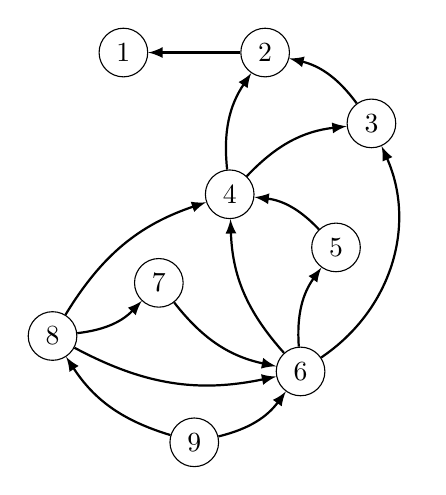
\begin{tikzpicture}[scale=0.9]
\node[draw, circle] (1) at (0,0) {$1$};
\node[draw, circle] (2) at (2,0) {$2$};
\node[draw, circle] (3) at (3.5,-1) {$3$};
\node[draw, circle] (4) at (1.5,-2) {$4$};
\node[draw, circle] (5) at (3,-2.75) {$5$};
\node[draw, circle] (6) at (2.5,-4.5) {$6$};
\node[draw, circle] (7) at (0.5,-3.25) {$7$};
\node[draw, circle] (8) at (-1,-4) {$8$};
\node[draw, circle] (9) at (1,-5.5) {$9$};

\path[draw,thick,->,>=latex] (2) -- (1);
\path[draw,thick,->,>=latex] (3) edge [bend right=20] (2);
\path[draw,thick,->,>=latex] (4) edge [bend left=20] (2);
\path[draw,thick,->,>=latex] (4) edge [bend left=20] (3);
\path[draw,thick,->,>=latex] (5) edge [bend right=20] (4);
\path[draw,thick,->,>=latex] (6) edge [bend left=20] (5);
\path[draw,thick,->,>=latex] (6) edge [bend left=20] (4);
\path[draw,thick,->,>=latex] (6) edge [bend right=40] (3);
\path[draw,thick,->,>=latex] (7) edge [bend right=20] (6);
\path[draw,thick,->,>=latex] (8) edge [bend right=20] (7);
\path[draw,thick,->,>=latex] (8) edge [bend right=20] (6);
\path[draw,thick,->,>=latex] (8) edge [bend left=20] (4);
\path[draw,thick,->,>=latex] (9) edge [bend left=20] (8);
\path[draw,thick,->,>=latex] (9) edge [bend right=20] (6);
\end{tikzpicture}
\end{center}

وضعیت پایانی در این بازی همواره وضعیت ۱ است،
که وضعیتی بازنده است، زیرا هیچ
حرکت معتبری وجود ندارد.
دسته‌بندی وضعیت‌های $1 \ldots 9$
به صورت زیر است:

\begin{center}
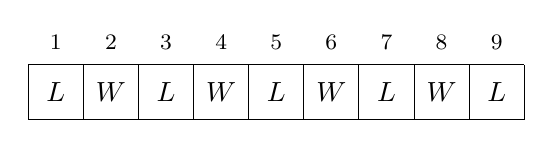
\begin{tikzpicture}[scale=0.7]
\draw (1,0) grid (10,1);

\node at (1.5,0.5) {$L$};
\node at (2.5,0.5) {$W$};
\node at (3.5,0.5) {$L$};
\node at (4.5,0.5) {$W$};
\node at (5.5,0.5) {$L$};
\node at (6.5,0.5) {$W$};
\node at (7.5,0.5) {$L$};
\node at (8.5,0.5) {$W$};
\node at (9.5,0.5) {$L$};

\footnotesize
\node at (1.5,1.4) {$1$};
\node at (2.5,1.4) {$2$};
\node at (3.5,1.4) {$3$};
\node at (4.5,1.4) {$4$};
\node at (5.5,1.4) {$5$};
\node at (6.5,1.4) {$6$};
\node at (7.5,1.4) {$7$};
\node at (8.5,1.4) {$8$};
\node at (9.5,1.4) {$9$};
\end{tikzpicture}
\end{center}

جالب توجه است که در این بازی،
تمام وضعیت‌های زوج وضعیت‌های برد
و تمام وضعیت‌های فرد وضعیت‌های باخت هستند.

\section{بازی نیم}

\index{بازی نیم}

\key{بازی نیم} (nim game) بازی ساده‌ای است که
نقش مهمی در نظریه بازی‌ها دارد،
زیرا بازی‌های بسیار دیگری را می‌توان با استفاده از
همین راهبرد انجام داد.
ابتدا روی نیم تمرکز می‌کنیم
و سپس این راهبرد را به بازی‌های دیگر
تعمیم می‌دهیم.

در نیم $n$ دسته وجود دارد
و هر دسته شامل تعدادی چوب است.
بازیکنان به نوبت حرکت می‌کنند
و در هر نوبت، بازیکن دسته‌ای را انتخاب می‌کند
که هنوز چوب دارد
و هر تعداد چوب دلخواه از آن برمی‌دارد.
برنده بازیکنی است که آخرین چوب را بردارد.

وضعیت‌ها در نیم به شکل
$[x_1,x_2,\ldots,x_n]$ هستند
که در آن $x_k$ نشان‌دهنده تعداد چوب‌های دسته $k$ است.
برای نمونه، $[10,12,5]$ یک بازی است که
در آن سه دسته با ۱۰، ۱۲ و ۵ چوب وجود دارد.
وضعیت $[0,0,\ldots,0]$ یک وضعیت باخت است،
زیرا امکان برداشتن هیچ چوبی وجود ندارد،
و این همواره وضعیت پایانی است.

\subsubsection{تحلیل}
\index{مجموع نیم}

مشخص می‌شود که می‌توانیم به‌سادگی
هر وضعیت نیم را با محاسبه
\key{مجموع نیم} $s = x_1 \oplus x_2 \oplus \cdots \oplus x_n$
دسته‌بندی کنیم،
که در آن $\oplus$ عملیات xor است\footnote{راهبرد بهینه
برای نیم در سال ۱۹۰۱ توسط C. L. Bouton منتشر شد \cite{bou01}.}.
وضعیت‌هایی که مجموع نیم آن‌ها برابر ۰ است وضعیت باخت
و بقیه وضعیت‌ها وضعیت برد هستند.
برای نمونه، مجموع نیم
$[10,12,5]$ برابر $10 \oplus 12 \oplus 5 = 3$ است،
بنابراین این وضعیت یک وضعیت برد است.

اما مجموع نیم چه ارتباطی با بازی نیم دارد؟
می‌توانیم این موضوع را با بررسی چگونگی تغییر
مجموع نیم هنگام تغییر وضعیت نیم توضیح دهیم.

\textit{وضعیت‌های باخت:}
وضعیت پایانی $[0,0,\ldots,0]$ یک وضعیت باخت است
و مجموع نیم آن برابر ۰ است، همان‌طور که انتظار می‌رفت.
در دیگر وضعیت‌های باخت، هر حرکتی به
یک وضعیت برد می‌انجامد، زیرا با تغییر یک مقدار $x_k$،
مجموع نیم نیز تغییر می‌کند، بنابراین مجموع نیم
پس از حرکت با ۰ متفاوت خواهد بود.

\textit{وضعیت‌های برد:}
می‌توانیم به یک وضعیت باخت حرکت کنیم اگر
دسته‌ای مانند $k$ وجود داشته باشد که $x_k \oplus s < x_k$ باشد.
در این حالت، می‌توانیم چوب‌هایی از
دسته $k$ برداریم به طوری که شامل $x_k \oplus s$ چوب شود،
که این به یک وضعیت باخت می‌انجامد.
همواره چنین دسته‌ای وجود دارد؛ جایی که $x_k$
در موقعیت چپ‌ترین بیت یکِ $s$، دارای بیت یک باشد.

به عنوان نمونه، وضعیت $[10,12,5]$ را در نظر بگیرید.
این وضعیت یک وضعیت برد است،
زیرا مجموع نیم آن برابر ۳ است.
بنابراین، باید حرکتی وجود داشته باشد که
به یک وضعیت باخت منتهی شود.
در ادامه چنین حرکتی را پیدا خواهیم کرد.

مجموع نیم (nim sum) این وضعیت بدین صورت است:

\begin{center}
\begin{tabular}{r|r}
10 & \texttt{1010} \\
12 & \texttt{1100} \\
5 & \texttt{0101} \\
\hline
3 & \texttt{0011} \\
\end{tabular}
\end{center}

در این حالت، کپه با ۱۰ چوب تنها کپه‌ای است که در جایگاه چپ‌ترین بیت یک در مجموع نیم، بیت یک دارد:

\begin{center}
\begin{tabular}{r|r}
10 & \texttt{10\underline{1}0} \\
12 & \texttt{1100} \\
5 & \texttt{0101} \\
\hline
3 & \texttt{00\underline{1}1} \\
\end{tabular}
\end{center}

اندازه جدید کپه باید $10 \oplus 3 = 9$ باشد، بنابراین فقط یک چوب حذف می‌کنیم. پس از این، وضعیت به $[9,12,5]$ تبدیل می‌شود که وضعیتی بازنده است:

\begin{center}
\begin{tabular}{r|r}
9 & \texttt{1001} \\
12 & \texttt{1100} \\
5 & \texttt{0101} \\
\hline
0 & \texttt{0000} \\
\end{tabular}
\end{center}

\subsubsection{بازی مزیر (Misère game)}

\index{misère game}

در یک \key{بازی مزیر}، هدف بازی برعکس است؛ یعنی بازیکنی که آخرین چوب را بردارد، بازی را می‌بازد. مشخص شده که بازی نیم مزیر را می‌توان به صورت بهینه تقریباً مشابه بازی استاندارد نیم انجام داد.

ایده این است که ابتدا بازی مزیر مانند بازی استاندارد انجام شود، اما در انتهای بازی راهبرد تغییر کند. راهبرد جدید در موقعیتی اعمال می‌شود که پس از حرکت بعدی، هر کپه حداکثر شامل یک چوب باشد.

در بازی استاندارد، باید حرکتی انتخاب شود که پس از آن تعداد زوجی از کپه‌های تک‌چوبی باقی بماند. اما در بازی مزیر، حرکتی انتخاب می‌شود که تعداد فردی از کپه‌های تک‌چوبی بر جای بماند.

این راهبرد کار می‌کند زیرا وضعیتی که راهبرد در آن تغییر می‌کند همواره در بازی رخ می‌دهد، و این وضعیت یک وضعیت برنده است، زیرا دقیقاً یک کپه دارد که بیش از یک چوب دارد، پس مجموع نیم آن صفر نیست.

\section{قضیه اسپرگ–گراندی (Sprague–Grundy theorem)}

\index{Sprague–Grundy theorem}

\key{قضیه اسپرگ–گراندی}\footnote{این قضیه به طور مستقل توسط آر. اسپرگ \cite{spr35} و پی. ام. گراندی \cite{gru39} کشف شد.} راهبرد استفاده‌شده در بازی نیم را برای تمام بازی‌هایی که شرایط زیر را برآورده کنند، تعمیم می‌دهد:

\begin{itemize}[noitemsep]
\item دو بازیکن به نوبت حرکت می‌کنند.
\item بازی شامل وضعیت‌ها است و حرکات ممکن در هر وضعیت به این که نوبت چه کسی است بستگی ندارد.
\item بازی زمانی پایان می‌یابد که یک بازیکن نتواند حرکتی انجام دهد.
\item بازی قطعاً دیر یا زود پایان می‌یابد.
\item بازیکنان اطلاعات کامل درباره وضعیت‌ها و حرکات مجاز دارند و هیچ تصادفی در بازی وجود ندارد.
\end{itemize}
ایده این است که برای هر وضعیت بازی یک عدد گراندی محاسبه شود که متناظر با تعداد چوب‌ها در یک کپه بازی نیم باشد. وقتی اعداد گراندی تمام وضعیت‌ها را بدانیم، می‌توانیم بازی را مانند بازی نیم انجام دهیم.

\subsubsection{اعداد گراندی}

\index{Grundy number}
\index{mex function}

\key{عدد گراندی} یک وضعیت بازی برابر است با
\[\textrm{mex}(\{g_1,g_2,\ldots,g_n\}),\]
که در آن $g_1,g_2,\ldots,g_n$ اعداد گراندی
وضعیت‌هایی هستند که می‌توان به آن‌ها حرکت کرد،
و تابع mex کوچک‌ترین عدد نامنفی را می‌دهد
که در مجموعه وجود ندارد.
به عنوان مثال، $\textrm{mex}(\{0,1,3\})=2$.
اگر حرکتی از یک وضعیت امکان‌پذیر نباشد،
عدد گراندی آن 0 است، زیرا
$\textrm{mex}(\emptyset)=0$.

برای نمونه، در گراف وضعیت
\begin{center}
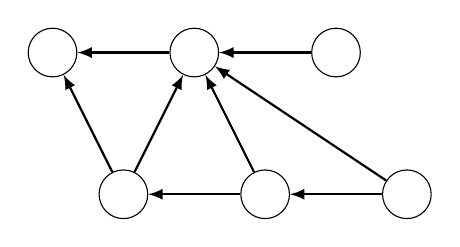
\begin{tikzpicture}[scale=0.9]
\node[draw, circle] (1) at (0,0) {\phantom{0}};
\node[draw, circle] (2) at (2,0) {\phantom{0}};
\node[draw, circle] (3) at (4,0) {\phantom{0}};
\node[draw, circle] (4) at (1,-2) {\phantom{0}};
\node[draw, circle] (5) at (3,-2) {\phantom{0}};
\node[draw, circle] (6) at (5,-2) {\phantom{0}};

\path[draw,thick,->,>=latex] (2) -- (1);
\path[draw,thick,->,>=latex] (3) -- (2);
\path[draw,thick,->,>=latex] (5) -- (4);
\path[draw,thick,->,>=latex] (6) -- (5);
\path[draw,thick,->,>=latex] (4) -- (1);
\path[draw,thick,->,>=latex] (4) -- (2);
\path[draw,thick,->,>=latex] (5) -- (2);
\path[draw,thick,->,>=latex] (6) -- (2);
\end{tikzpicture}
\end{center}
اعداد گراندی به صورت زیر هستند:
\begin{center}
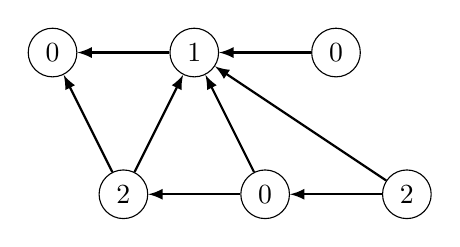
\begin{tikzpicture}[scale=0.9]
\node[draw, circle] (1) at (0,0) {0};
\node[draw, circle] (2) at (2,0) {1};
\node[draw, circle] (3) at (4,0) {0};
\node[draw, circle] (4) at (1,-2) {2};
\node[draw, circle] (5) at (3,-2) {0};
\node[draw, circle] (6) at (5,-2) {2};

\path[draw,thick,->,>=latex] (2) -- (1);
\path[draw,thick,->,>=latex] (3) -- (2);
\path[draw,thick,->,>=latex] (5) -- (4);
\path[draw,thick,->,>=latex] (6) -- (5);
\path[draw,thick,->,>=latex] (4) -- (1);
\path[draw,thick,->,>=latex] (4) -- (2);
\path[draw,thick,->,>=latex] (5) -- (2);
\path[draw,thick,->,>=latex] (6) -- (2);
\end{tikzpicture}
\end{center}
عدد گراندی یک وضعیت بازنده برابر 0 است،
و عدد گراندی یک وضعیت برنده
عددی مثبت است.

عدد گراندی یک وضعیت متناظر است با
تعداد چوب‌ها در یک دسته نیم.
اگر عدد گراندی 0 باشد، فقط می‌توان به
وضعیت‌هایی رفت که عدد گراندی آن‌ها مثبت است،
و اگر عدد گراندی $x>0$ باشد، می‌توان به
وضعیت‌هایی رفت که اعداد گراندی آن‌ها شامل همه اعداد
$0,1,\ldots,x-1$ است.

به عنوان مثال، بازی‌ای را در نظر بگیرید که در آن
بازیکنان مهره‌ای را درون یک ماز حرکت می‌دهند.
هر خانه ماز یا کف است یا دیوار.
در هر نوبت، بازیکن باید مهره را
تعدادی گام به چپ یا بالا حرکت دهد.
برنده بازی بازیکنی است که
آخرین حرکت را انجام دهد.

تصویر زیر یک وضعیت آغازین ممکن از بازی
را نشان می‌دهد، که در آن @ مهره را مشخص می‌کند و *
خانه‌ای را نشان می‌دهد که مهره می‌تواند به آن حرکت کند.

\begin{center}
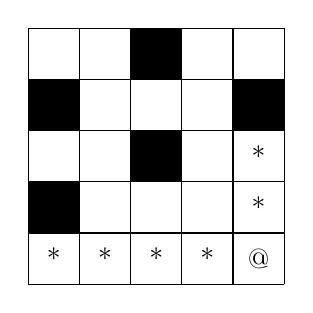
\begin{tikzpicture}[scale=.65]
  \begin{scope}
    \fill [color=black] (0, 1) rectangle (1, 2);
    \fill [color=black] (0, 3) rectangle (1, 4);
    \fill [color=black] (2, 2) rectangle (3, 3);
    \fill [color=black] (2, 4) rectangle (3, 5);
    \fill [color=black] (4, 3) rectangle (5, 4);

    \draw (0, 0) grid (5, 5);
    
    \node at (4.5,0.5) {@};
    \node at (3.5,0.5) {*};
    \node at (2.5,0.5) {*};
    \node at (1.5,0.5) {*};
    \node at (0.5,0.5) {*};
    \node at (4.5,1.5) {*};
    \node at (4.5,2.5) {*};
    
  \end{scope}
\end{tikzpicture}
\end{center}

وضعیت‌های بازی، تمام خانه‌های خالی
مارپیچ هستند.
در مارپیچ بالا، اعداد گراندی
به این صورت است:

\begin{center}
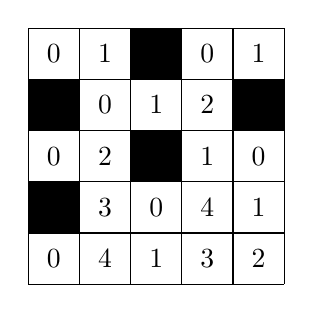
\begin{tikzpicture}[scale=.65]
  \begin{scope}
    \fill [color=black] (0, 1) rectangle (1, 2);
    \fill [color=black] (0, 3) rectangle (1, 4);
    \fill [color=black] (2, 2) rectangle (3, 3);
    \fill [color=black] (2, 4) rectangle (3, 5);
    \fill [color=black] (4, 3) rectangle (5, 4);

    \draw (0, 0) grid (5, 5);
    
    \node at (0.5,4.5) {0};
    \node at (1.5,4.5) {1};
    \node at (2.5,4.5) {};
    \node at (3.5,4.5) {0};
    \node at (4.5,4.5) {1};

    \node at (0.5,3.5) {};
    \node at (1.5,3.5) {0};
    \node at (2.5,3.5) {1};
    \node at (3.5,3.5) {2};
    \node at (4.5,3.5) {};

    \node at (0.5,2.5) {0};
    \node at (1.5,2.5) {2};
    \node at (2.5,2.5) {};
    \node at (3.5,2.5) {1};
    \node at (4.5,2.5) {0};

    \node at (0.5,1.5) {};
    \node at (1.5,1.5) {3};
    \node at (2.5,1.5) {0};
    \node at (3.5,1.5) {4};
    \node at (4.5,1.5) {1};

    \node at (0.5,0.5) {0};
    \node at (1.5,0.5) {4};
    \node at (2.5,0.5) {1};
    \node at (3.5,0.5) {3};
    \node at (4.5,0.5) {2};
  \end{scope}
\end{tikzpicture}
\end{center}

بنابراین، هر وضعیت بازی مارپیچ
معادل یک دسته در بازی نیم است.
برای نمونه، عدد گراندی خانه گوشه پایین‌راست برابر ۲ است،
پس وضعیتی برنده است.
با چهار گام حرکت به چپ یا
دو گام به بالا،
می‌توان به یک وضعیت بازنده رسید و بازی را برد.

برخلاف بازی نیم اصلی،
امکان رفتن به وضعیتی با عدد گراندی
بزرگ‌تر از وضعیت فعلی وجود دارد.
اما حریف همیشه حرکتی برای خنثی‌سازی دارد،
پس فرار از وضعیت بازنده ناممکن است.

\subsubsection{زیربازی‌ها}

فرض بازی شامل چند زیربازی است؛
در هر نوبت، بازیکن نخست یک زیربازی، سپس حرکتی در آن انتخاب می‌کند.
پایان بازی زمانی است که هیچ حرکتی در هیچ زیربازی ممکن نباشد.

در این حالت، عدد گراندی کل بازی،
حاصل‌جمع نیم اعداد گراندی زیربازی‌ها است.
بازی با محاسبه اعداد گراندی زیربازی‌ها و جمع نیم آن‌ها،
مانند بازی نیم اجرا می‌شود.

برای مثال، یک بازی با سه مارپیچ را در نظر بگیرید.
در هر نوبت، بازیکن یک مارپیچ را انتخاب کرده
و مهره را در آن جابه‌جا می‌کند.
فرض وضعیت اولیه بازی چنین است:

\begin{center}
\begin{tabular}{ccc}
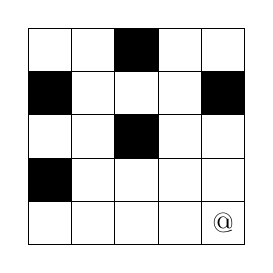
\begin{tikzpicture}[scale=.55]
  \begin{scope}
    \fill [color=black] (0, 1) rectangle (1, 2);
    \fill [color=black] (0, 3) rectangle (1, 4);
    \fill [color=black] (2, 2) rectangle (3, 3);
    \fill [color=black] (2, 4) rectangle (3, 5);
    \fill [color=black] (4, 3) rectangle (5, 4);

    \draw (0, 0) grid (5, 5);

    \node at (4.5,0.5) {@};

    \end{scope}
\end{tikzpicture}
&
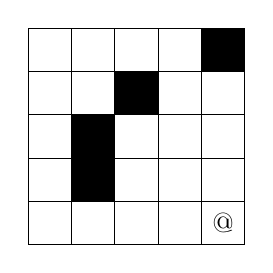
\begin{tikzpicture}[scale=.55]
  \begin{scope}
    \fill [color=black] (1, 1) rectangle (2, 3);
    \fill [color=black] (2, 3) rectangle (3, 4);
    \fill [color=black] (4, 4) rectangle (5, 5);

    \draw (0, 0) grid (5, 5);
    
    \node at (4.5,0.5) {@};

  \end{scope}
\end{tikzpicture}
&
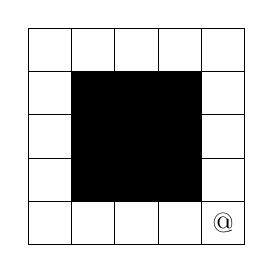
\begin{tikzpicture}[scale=.55]
  \begin{scope}
    \fill [color=black] (1, 1) rectangle (4, 4);

    \draw (0, 0) grid (5, 5);
    
    \node at (4.5,0.5) {@};
  \end{scope}
\end{tikzpicture}
\end{tabular}
\end{center}

اعداد گراندی برای مازها به صورت زیر هستند:

\begin{center}
\begin{tabular}{ccc}
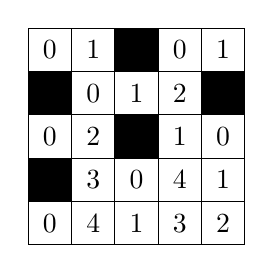
\begin{tikzpicture}[scale=.55]
  \begin{scope}
    \fill [color=black] (0, 1) rectangle (1, 2);
    \fill [color=black] (0, 3) rectangle (1, 4);
    \fill [color=black] (2, 2) rectangle (3, 3);
    \fill [color=black] (2, 4) rectangle (3, 5);
    \fill [color=black] (4, 3) rectangle (5, 4);

    \draw (0, 0) grid (5, 5);

    \node at (0.5,4.5) {0};
    \node at (1.5,4.5) {1};
    \node at (2.5,4.5) {};
    \node at (3.5,4.5) {0};
    \node at (4.5,4.5) {1};

    \node at (0.5,3.5) {};
    \node at (1.5,3.5) {0};
    \node at (2.5,3.5) {1};
    \node at (3.5,3.5) {2};
    \node at (4.5,3.5) {};

    \node at (0.5,2.5) {0};
    \node at (1.5,2.5) {2};
    \node at (2.5,2.5) {};
    \node at (3.5,2.5) {1};
    \node at (4.5,2.5) {0};

    \node at (0.5,1.5) {};
    \node at (1.5,1.5) {3};
    \node at (2.5,1.5) {0};
    \node at (3.5,1.5) {4};
    \node at (4.5,1.5) {1};

    \node at (0.5,0.5) {0};
    \node at (1.5,0.5) {4};
    \node at (2.5,0.5) {1};
    \node at (3.5,0.5) {3};
    \node at (4.5,0.5) {2};
    \end{scope}
\end{tikzpicture}
&
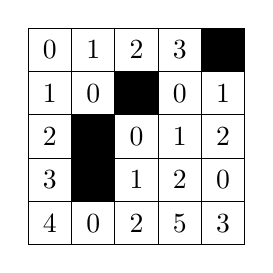
\begin{tikzpicture}[scale=.55]
  \begin{scope}
    \fill [color=black] (1, 1) rectangle (2, 3);
    \fill [color=black] (2, 3) rectangle (3, 4);
    \fill [color=black] (4, 4) rectangle (5, 5);

    \draw (0, 0) grid (5, 5);

    \node at (0.5,4.5) {0};
    \node at (1.5,4.5) {1};
    \node at (2.5,4.5) {2};
    \node at (3.5,4.5) {3};
    \node at (4.5,4.5) {};

    \node at (0.5,3.5) {1};
    \node at (1.5,3.5) {0};
    \node at (2.5,3.5) {};
    \node at (3.5,3.5) {0};
    \node at (4.5,3.5) {1};

    \node at (0.5,2.5) {2};
    \node at (1.5,2.5) {};
    \node at (2.5,2.5) {0};
    \node at (3.5,2.5) {1};
    \node at (4.5,2.5) {2};

    \node at (0.5,1.5) {3};
    \node at (1.5,1.5) {};
    \node at (2.5,1.5) {1};
    \node at (3.5,1.5) {2};
    \node at (4.5,1.5) {0};

    \node at (0.5,0.5) {4};
    \node at (1.5,0.5) {0};
    \node at (2.5,0.5) {2};
    \node at (3.5,0.5) {5};
    \node at (4.5,0.5) {3};
  \end{scope}
\end{tikzpicture}
&
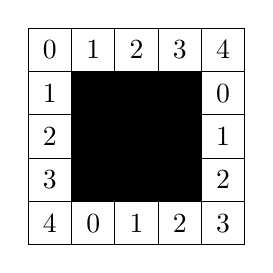
\begin{tikzpicture}[scale=.55]
  \begin{scope}
    \fill [color=black] (1, 1) rectangle (4, 4);

    \draw (0, 0) grid (5, 5);

    \node at (0.5,4.5) {0};
    \node at (1.5,4.5) {1};
    \node at (2.5,4.5) {2};
    \node at (3.5,4.5) {3};
    \node at (4.5,4.5) {4};

    \node at (0.5,3.5) {1};
    \node at (1.5,3.5) {};
    \node at (2.5,3.5) {};
    \node at (3.5,3.5) {};
    \node at (4.5,3.5) {0};

    \node at (0.5,2.5) {2};
    \node at (1.5,2.5) {};
    \node at (2.5,2.5) {};
    \node at (3.5,2.5) {};
    \node at (4.5,2.5) {1};

    \node at (0.5,1.5) {3};
    \node at (1.5,1.5) {};
    \node at (2.5,1.5) {};
    \node at (3.5,1.5) {};
    \node at (4.5,1.5) {2};

    \node at (0.5,0.5) {4};
    \node at (1.5,0.5) {0};
    \node at (2.5,0.5) {1};
    \node at (3.5,0.5) {2};
    \node at (4.5,0.5) {3};
  \end{scope}
\end{tikzpicture}
\end{tabular}
\end{center}

در وضعیت اولیه، مجموع نیم اعداد گراندی برابر $2 \oplus 3 \oplus 3 = 2$ است، بنابراین بازیکن اول می‌تواند بازی را ببرد. یک حرکت بهینه، دو گام حرکت به سمت بالا در هزارتوی اول است که مجموع نیم $0 \oplus 3 \oplus 3 = 0$ را تولید می‌کند.

\subsubsection{بازی گراندی}

گاهی یک حرکت در بازی، آن را به زیربازی‌های مستقل از یکدیگر تقسیم می‌کند. در این حالت، عدد گراندی بازی برابر است با:

\[\textrm{mex}(\{g_1, g_2, \ldots, g_n \}),\]
که $n$ تعداد حرکت‌های ممکن است و
\[g_k = a_{k,1} \oplus a_{k,2} \oplus \ldots \oplus a_{k,m},\]
به طوری که حرکت $k$ زیربازی‌هایی با اعداد گراندی $a_{k,1},a_{k,2},\ldots,a_{k,m}$ ایجاد می‌کند.

\index{Grundy's game}

نمونه‌ای از چنین بازی‌هایی، \key{بازی گراندی} است. در ابتدا، یک دسته شامل $n$ چوب وجود دارد. در هر نوبت، بازیکن یک دسته را انتخاب کرده و آن را به دو دسته ناتهی با اندازه‌های متفاوت تقسیم می‌کند. بازیکنی که آخرین حرکت را انجام دهد برنده بازی است.

فرض کنید $f(n)$ عدد گراندی دسته‌ای با $n$ چوب باشد. عدد گراندی با بررسی تمام روش‌های تقسیم دسته به دو دسته محاسبه می‌شود. برای مثال، وقتی $n=8$ است، حالت‌های ممکن $1+7$، $2+6$ و $3+5$ هستند، پس:
\[f(8)=\textrm{mex}(\{f(1) \oplus f(7), f(2) \oplus f(6), f(3) \oplus f(5)\}).\]

در این بازی، مقدار $f(n)$ بر اساس مقادیر $f(1),\ldots,f(n-1)$ به دست می‌آید. حالت‌های پایه $f(1)=f(2)=0$ هستند، زیرا تقسیم دسته‌های ۱ و ۲ چوبی ممکن نیست. نخستین اعداد گراندی عبارتند از:
\[
\begin{array}{lcl}
f(1) & = & 0 \\
f(2) & = & 0 \\
f(3) & = & 1 \\
f(4) & = & 0 \\
f(5) & = & 2 \\
f(6) & = & 1 \\
f(7) & = & 0 \\
f(8) & = & 2 \\
\end{array}
\]
عدد گراندی برای $n=8$ برابر ۲ است، بنابراین بردن بازی ممکن است. حرکت برنده، ساخت دسته‌های $1+7$ است، زیرا $f(1) \oplus f(7) = 0$.